\begin{figure}
    \centering
    \begin{minipage}{0.45\textwidth}
        \centering
        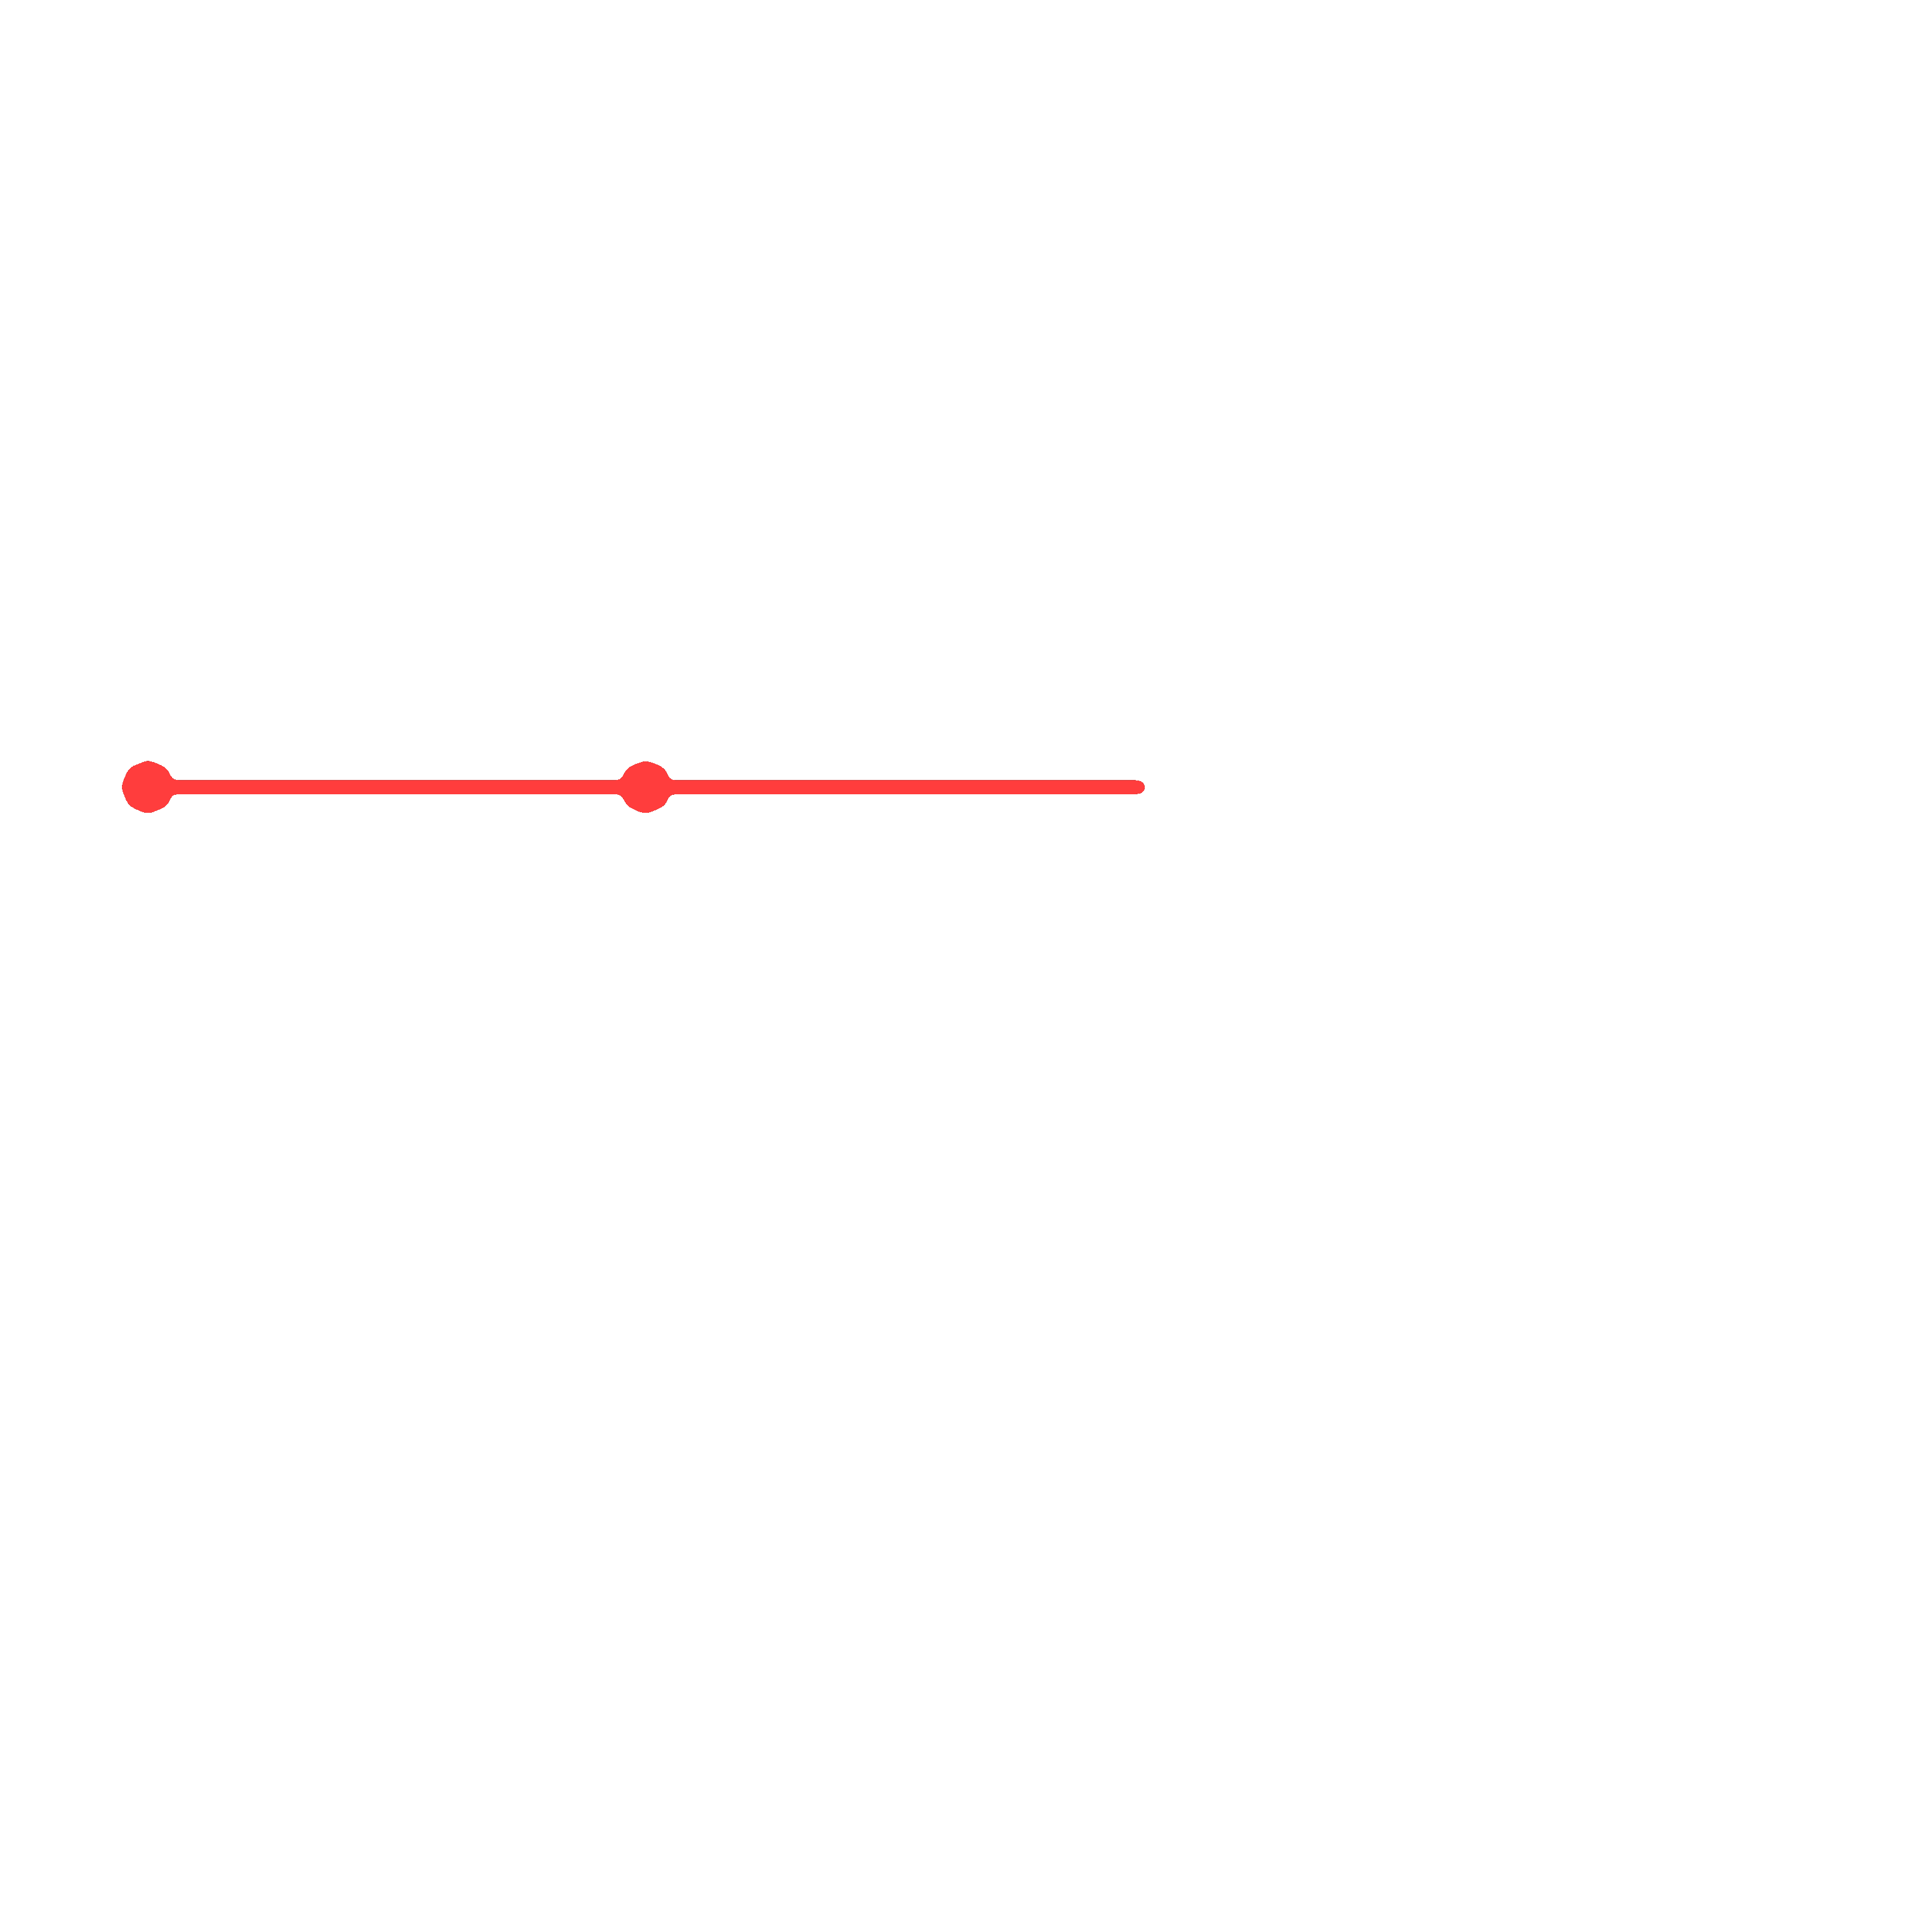
\includegraphics[width=\textwidth]{papers/doppelpendel/images/pendel_stand_90.png}
    \end{minipage}
    \hfill
    \begin{minipage}{0.45\textwidth}
        \centering
        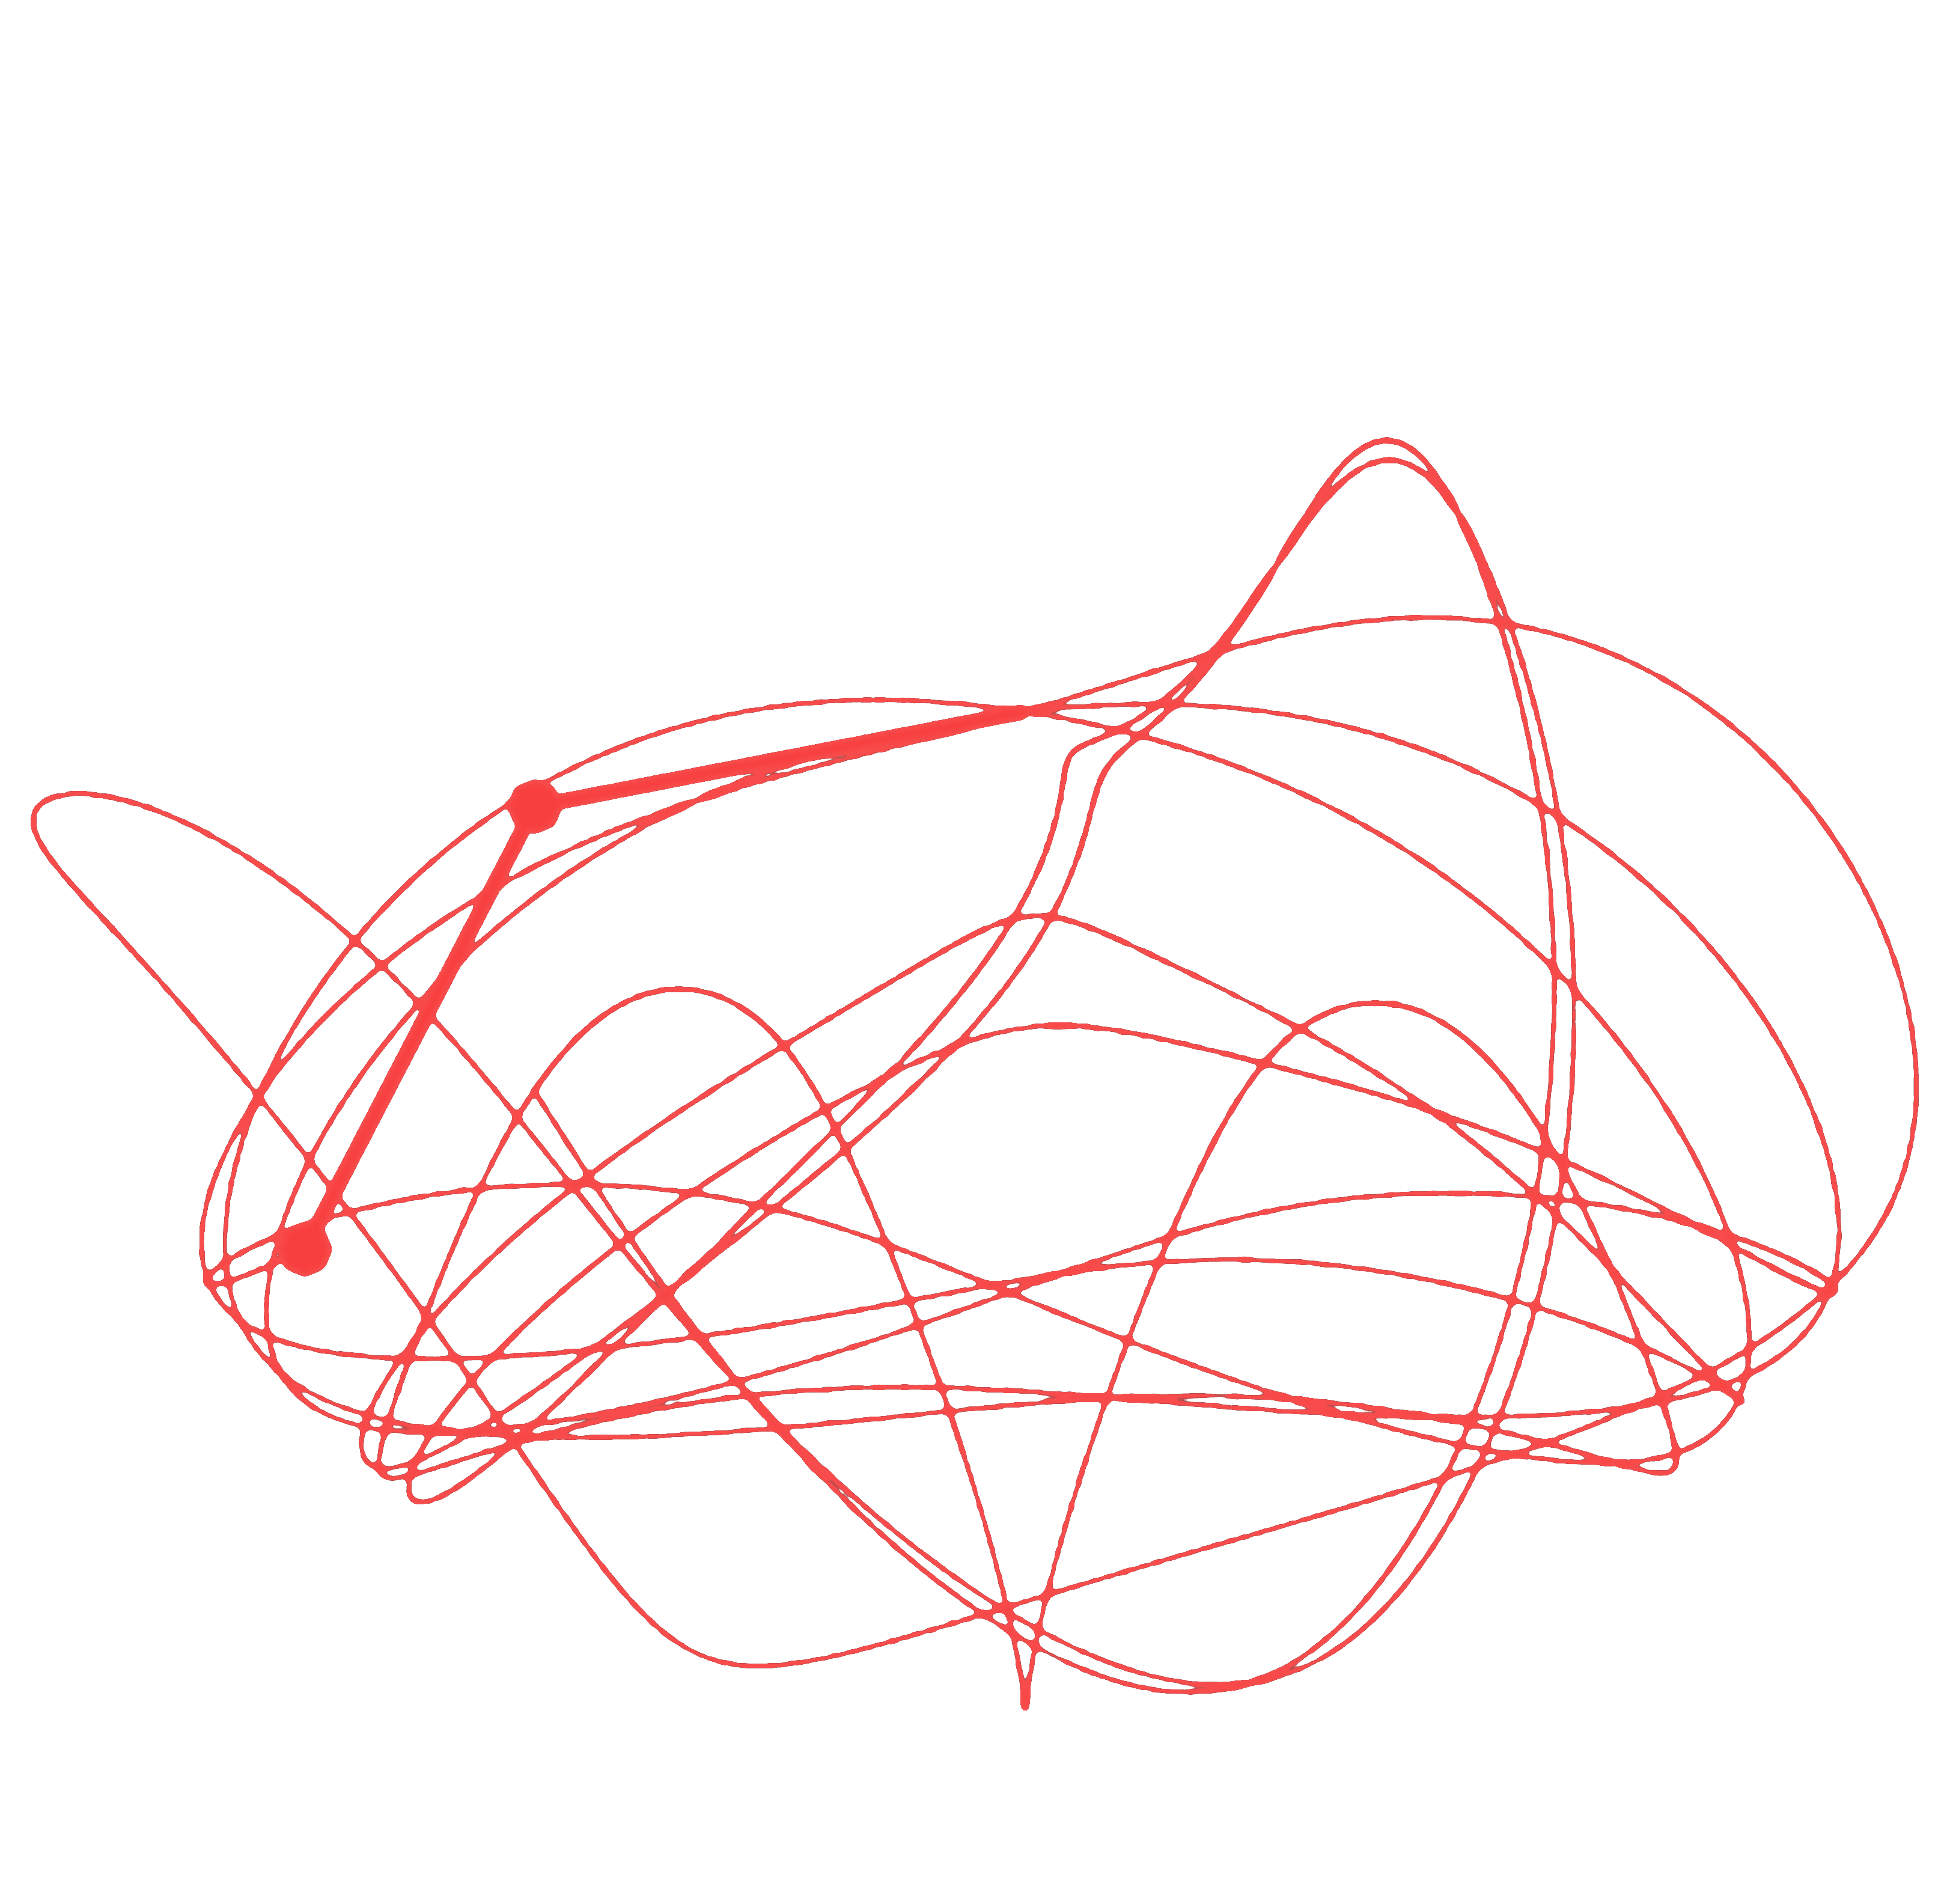
\includegraphics[width=\textwidth]{papers/doppelpendel/images/pendel_spur_90.png}
    \end{minipage}
    \caption{Pendel mit der Anfangsbedingung 90°.}
    \label{fig:pendel_bei_90}
    \centering
    \begin{minipage}{0.45\textwidth}
        \centering
        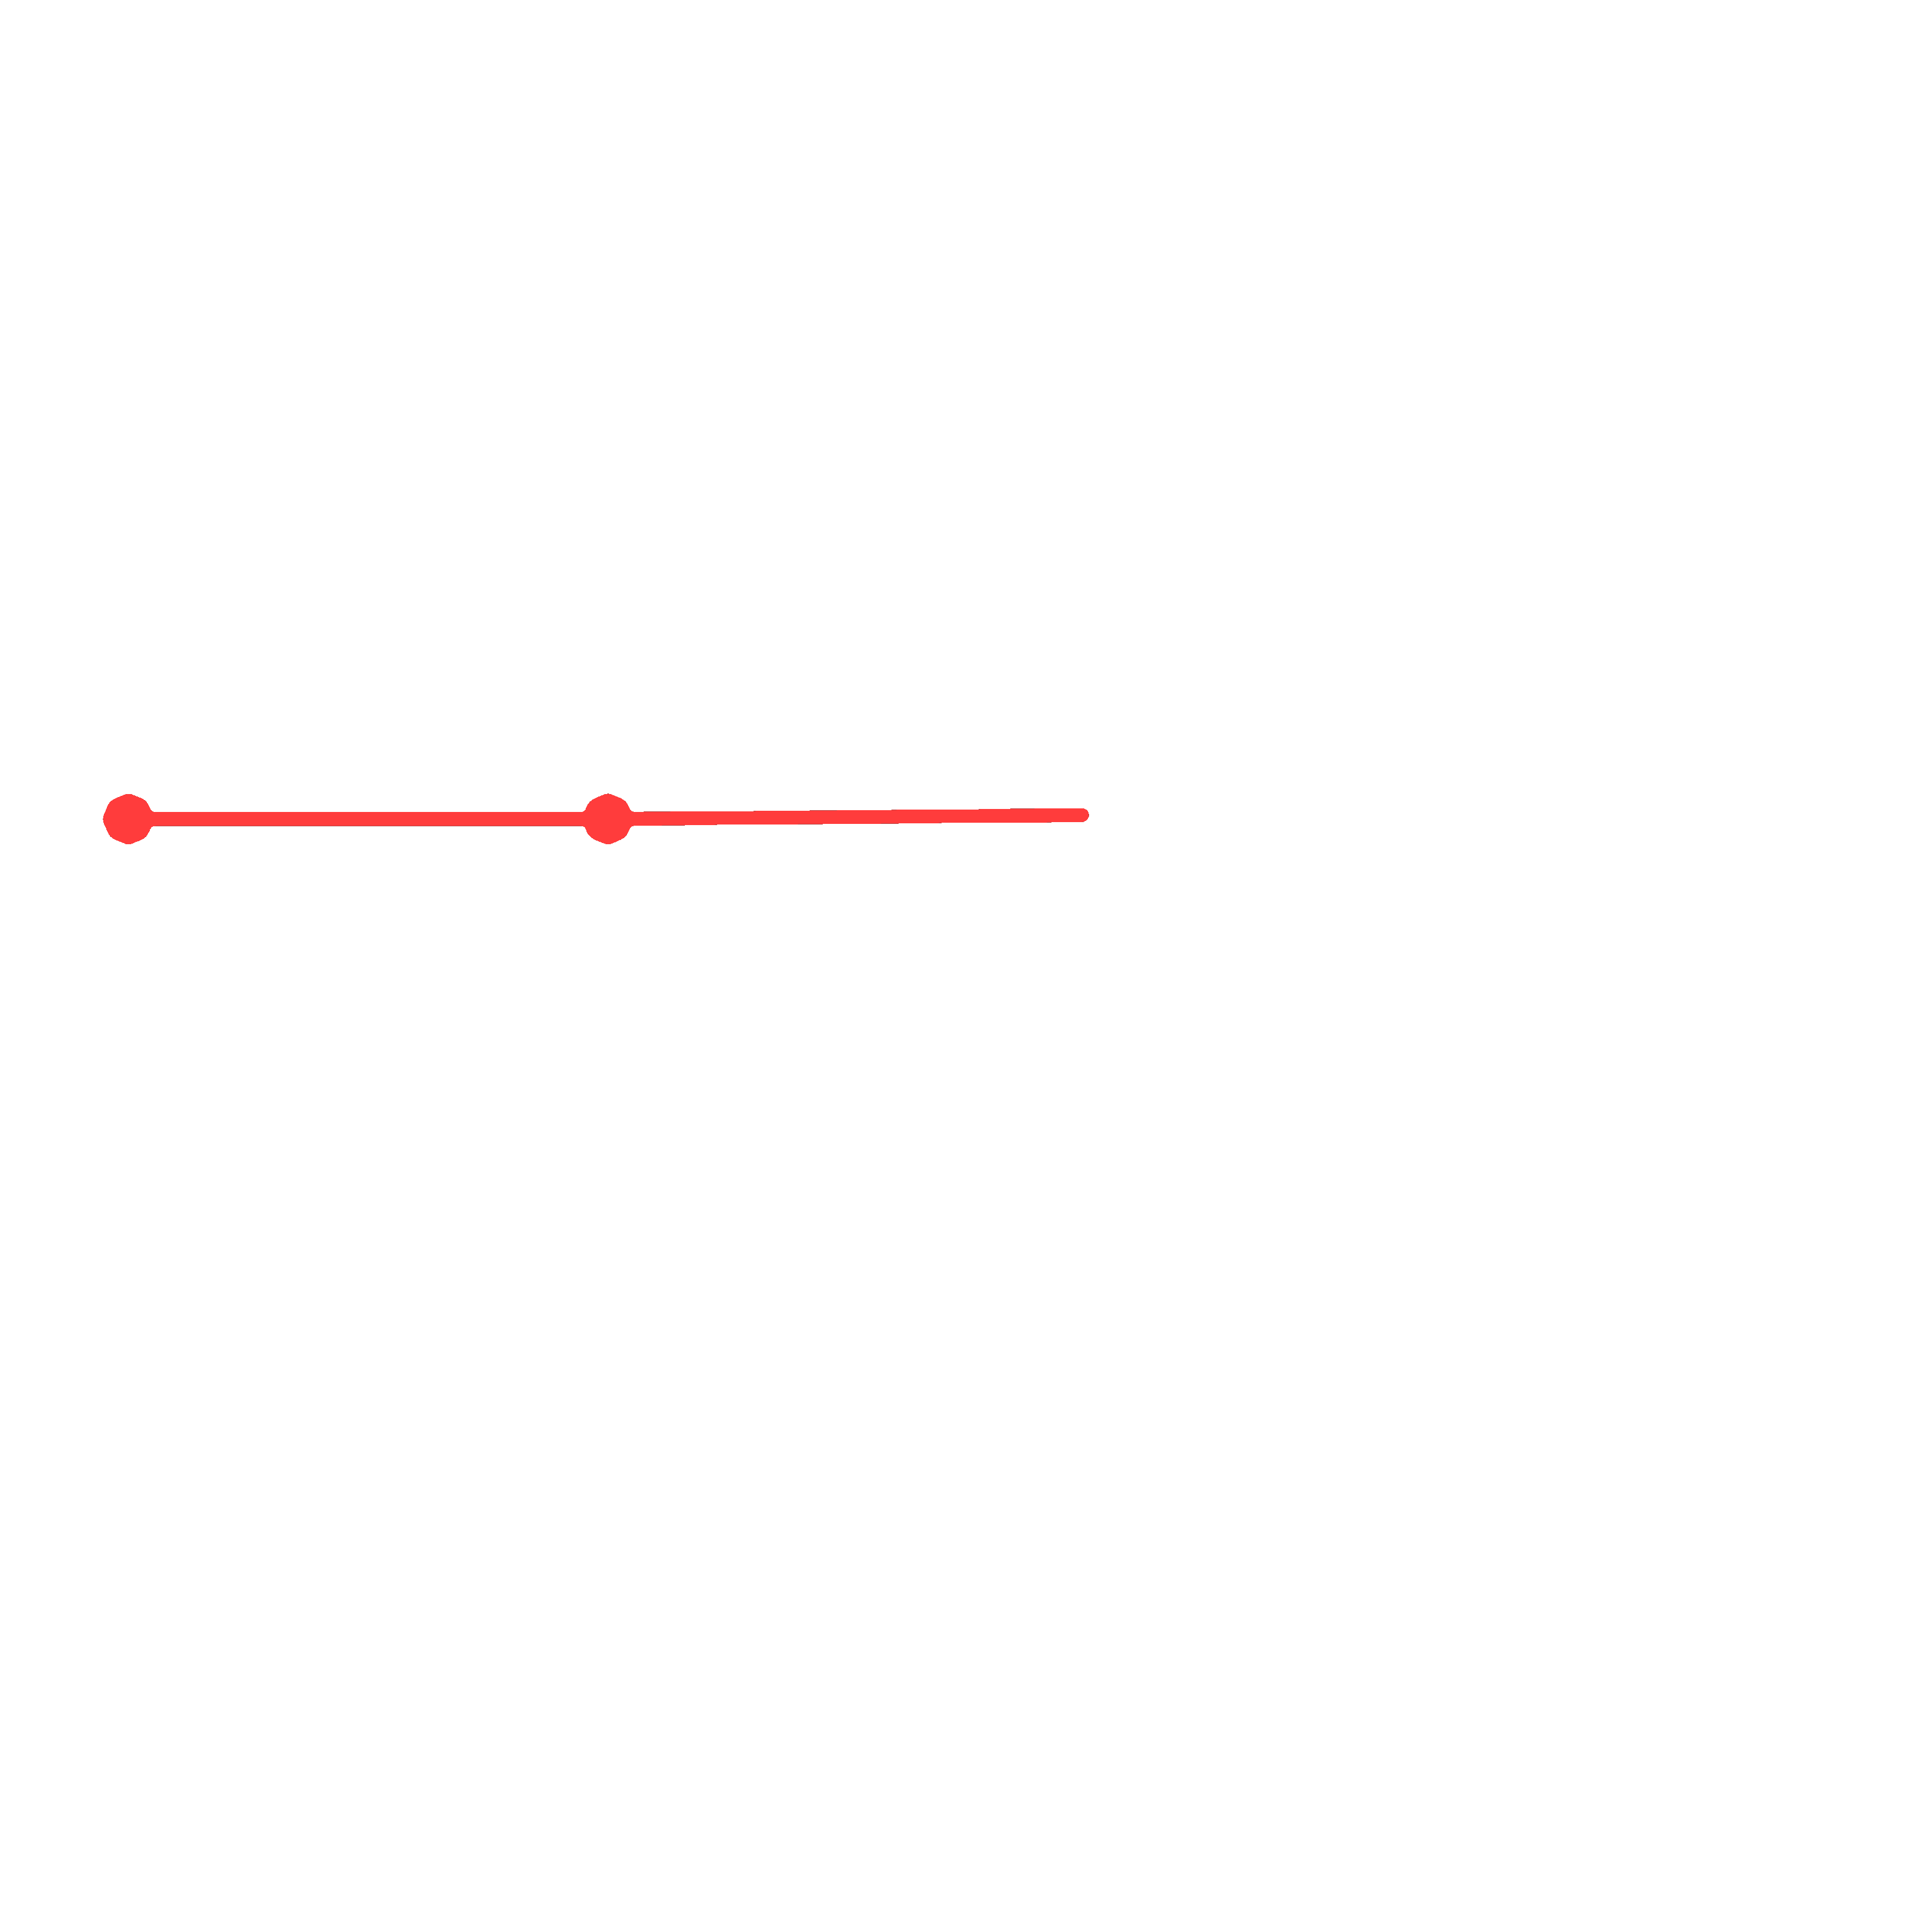
\includegraphics[width=\textwidth]{papers/doppelpendel/images/pendel_stand_kleiner_90.png}
    \end{minipage}
    \hfill
    \begin{minipage}{0.45\textwidth}
        \centering
        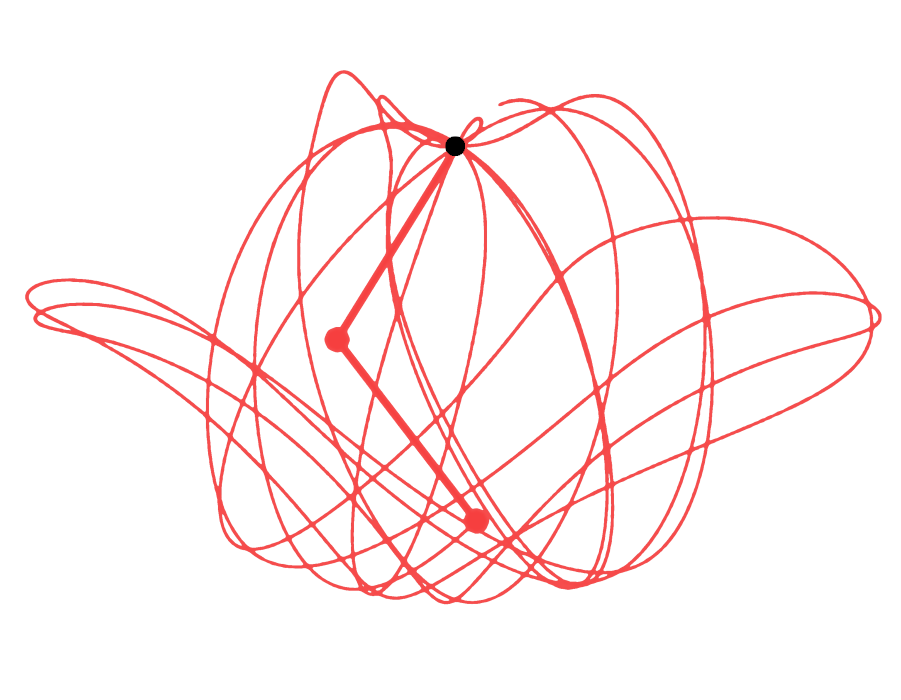
\includegraphics[width=\textwidth]{papers/doppelpendel/images/pendel_spur_kleiner_90.png}
    \end{minipage}
    \caption{Anfangsbedingung der Winkel ist kaum sichtbar kleiner als 90°.}
    \label{fig:pendel_bei_weniger_90}
    \centering
    \begin{minipage}{0.45\textwidth}
        \centering
        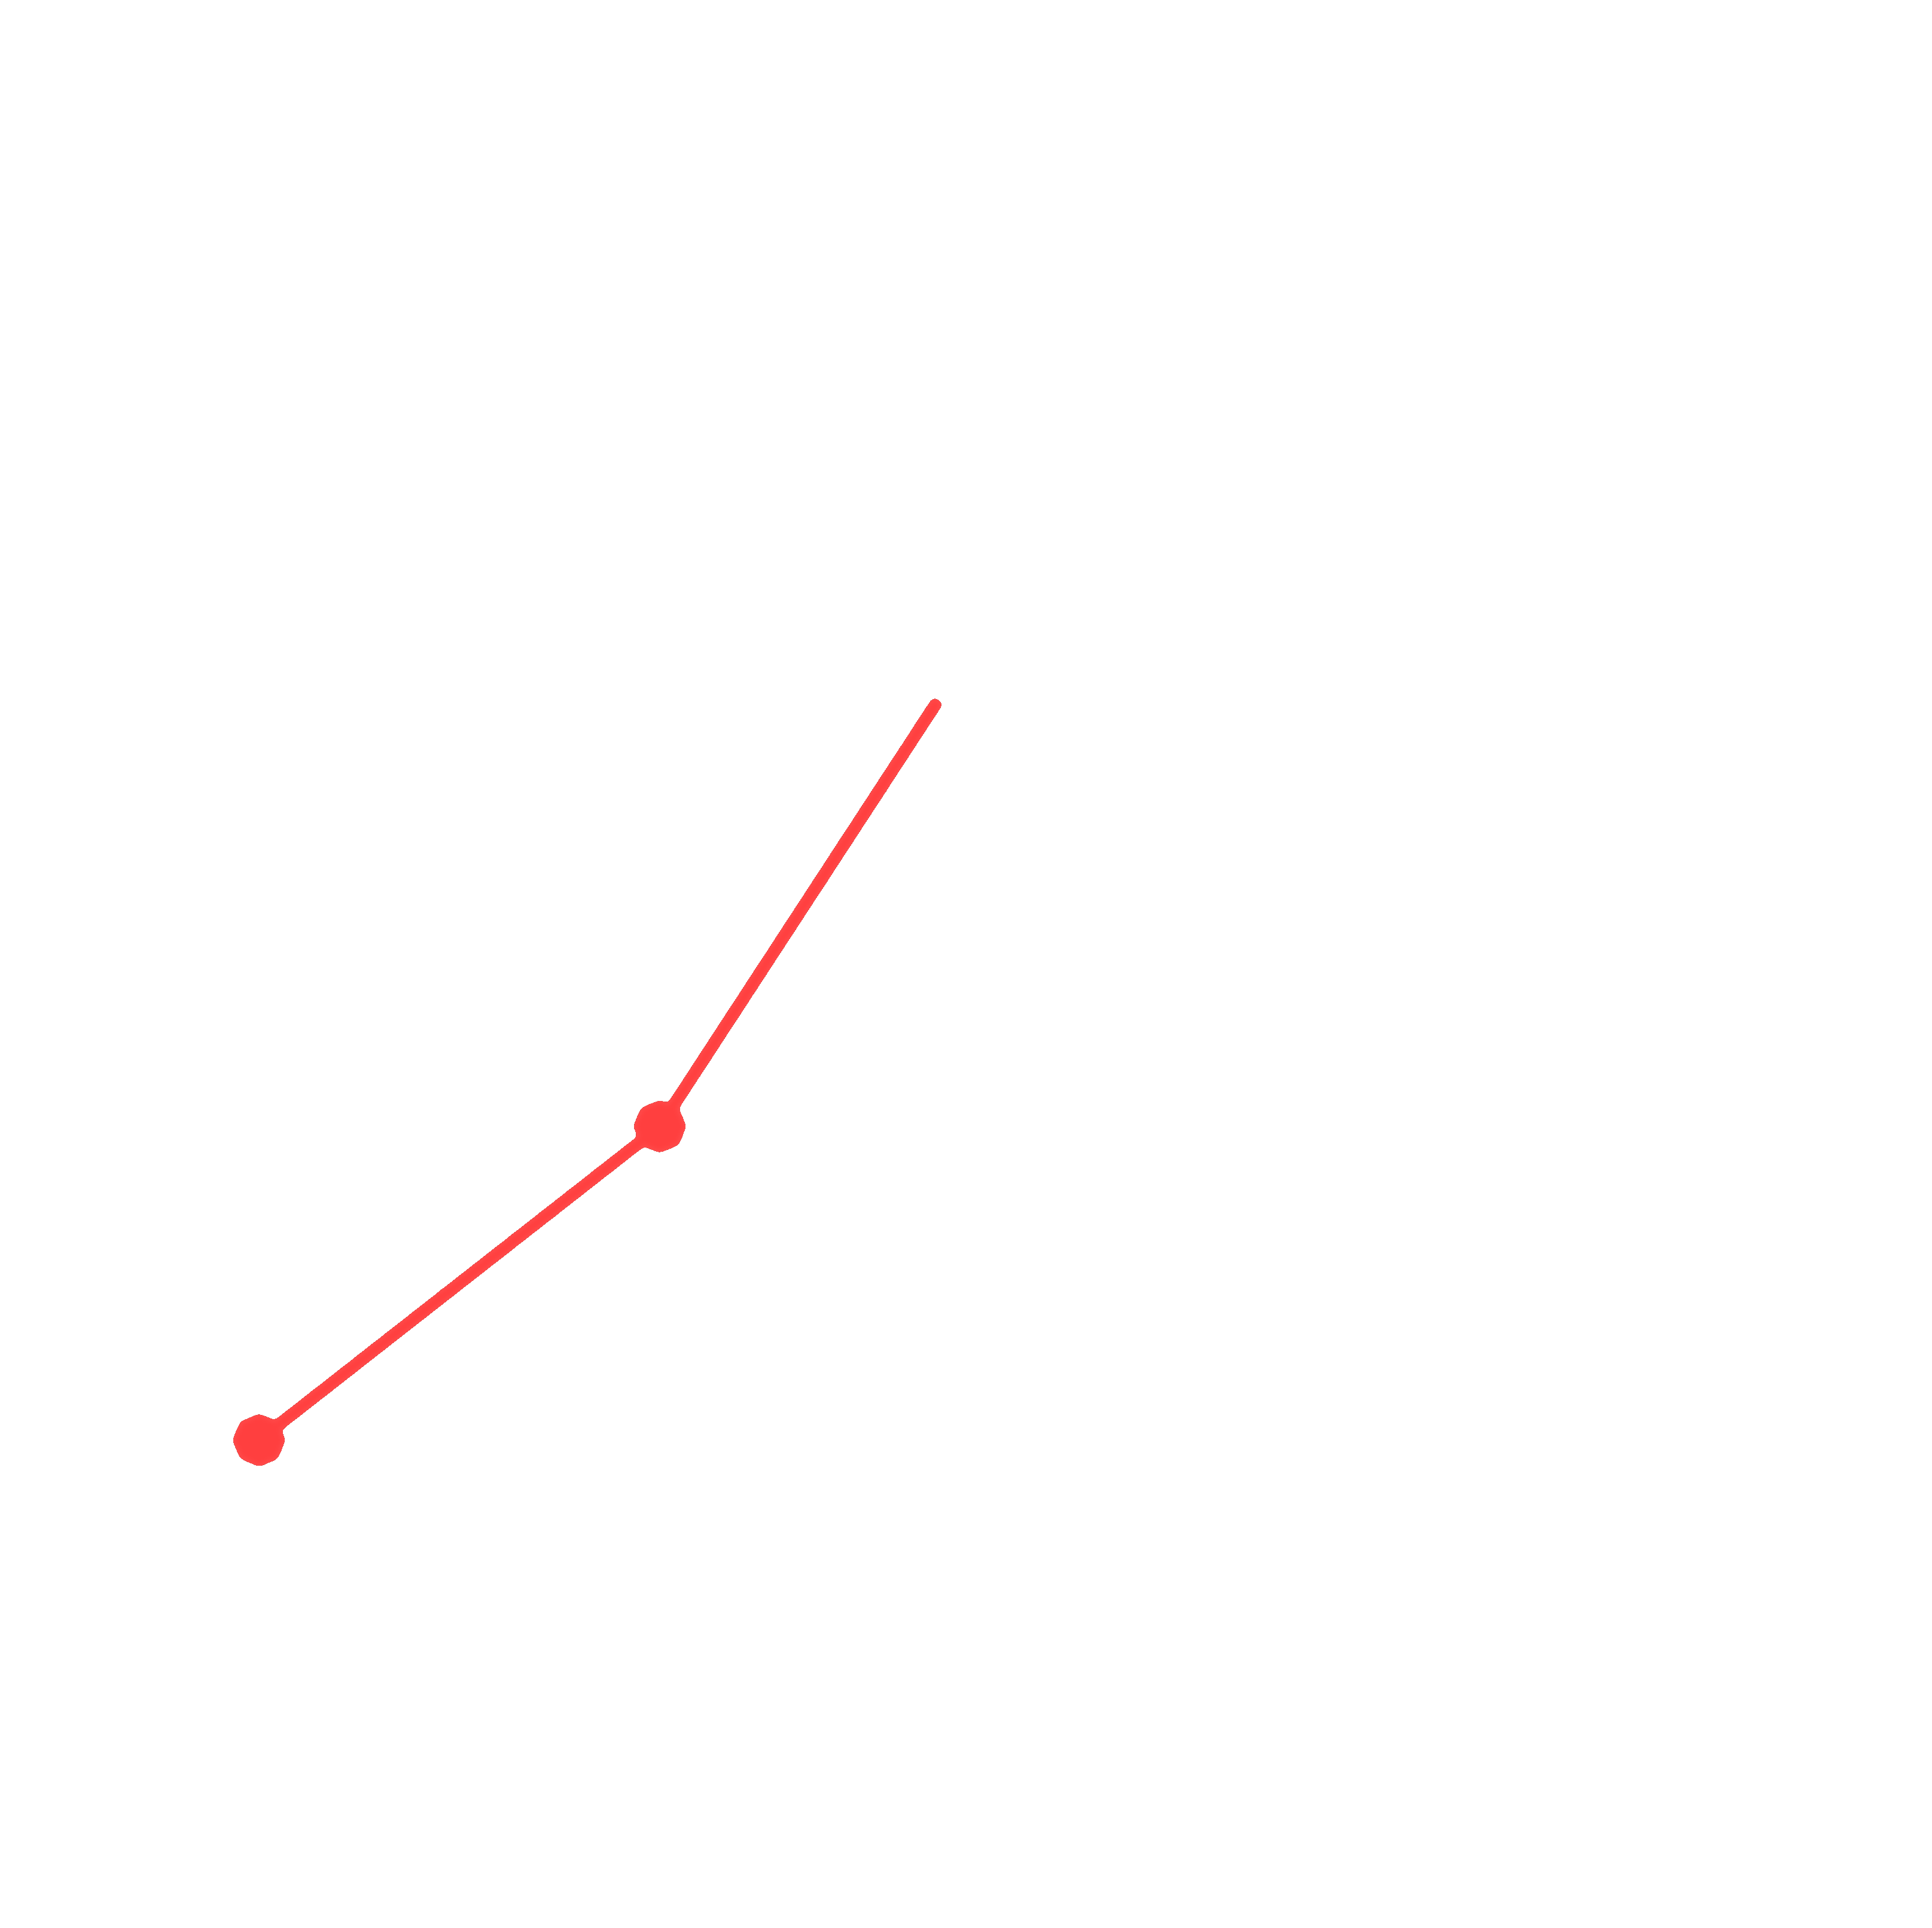
\includegraphics[width=\textwidth]{papers/doppelpendel/images/pendel_stand_nichtchaotisch.png}
    \end{minipage}
    \hfill
    \begin{minipage}{0.45\textwidth}
        \centering
        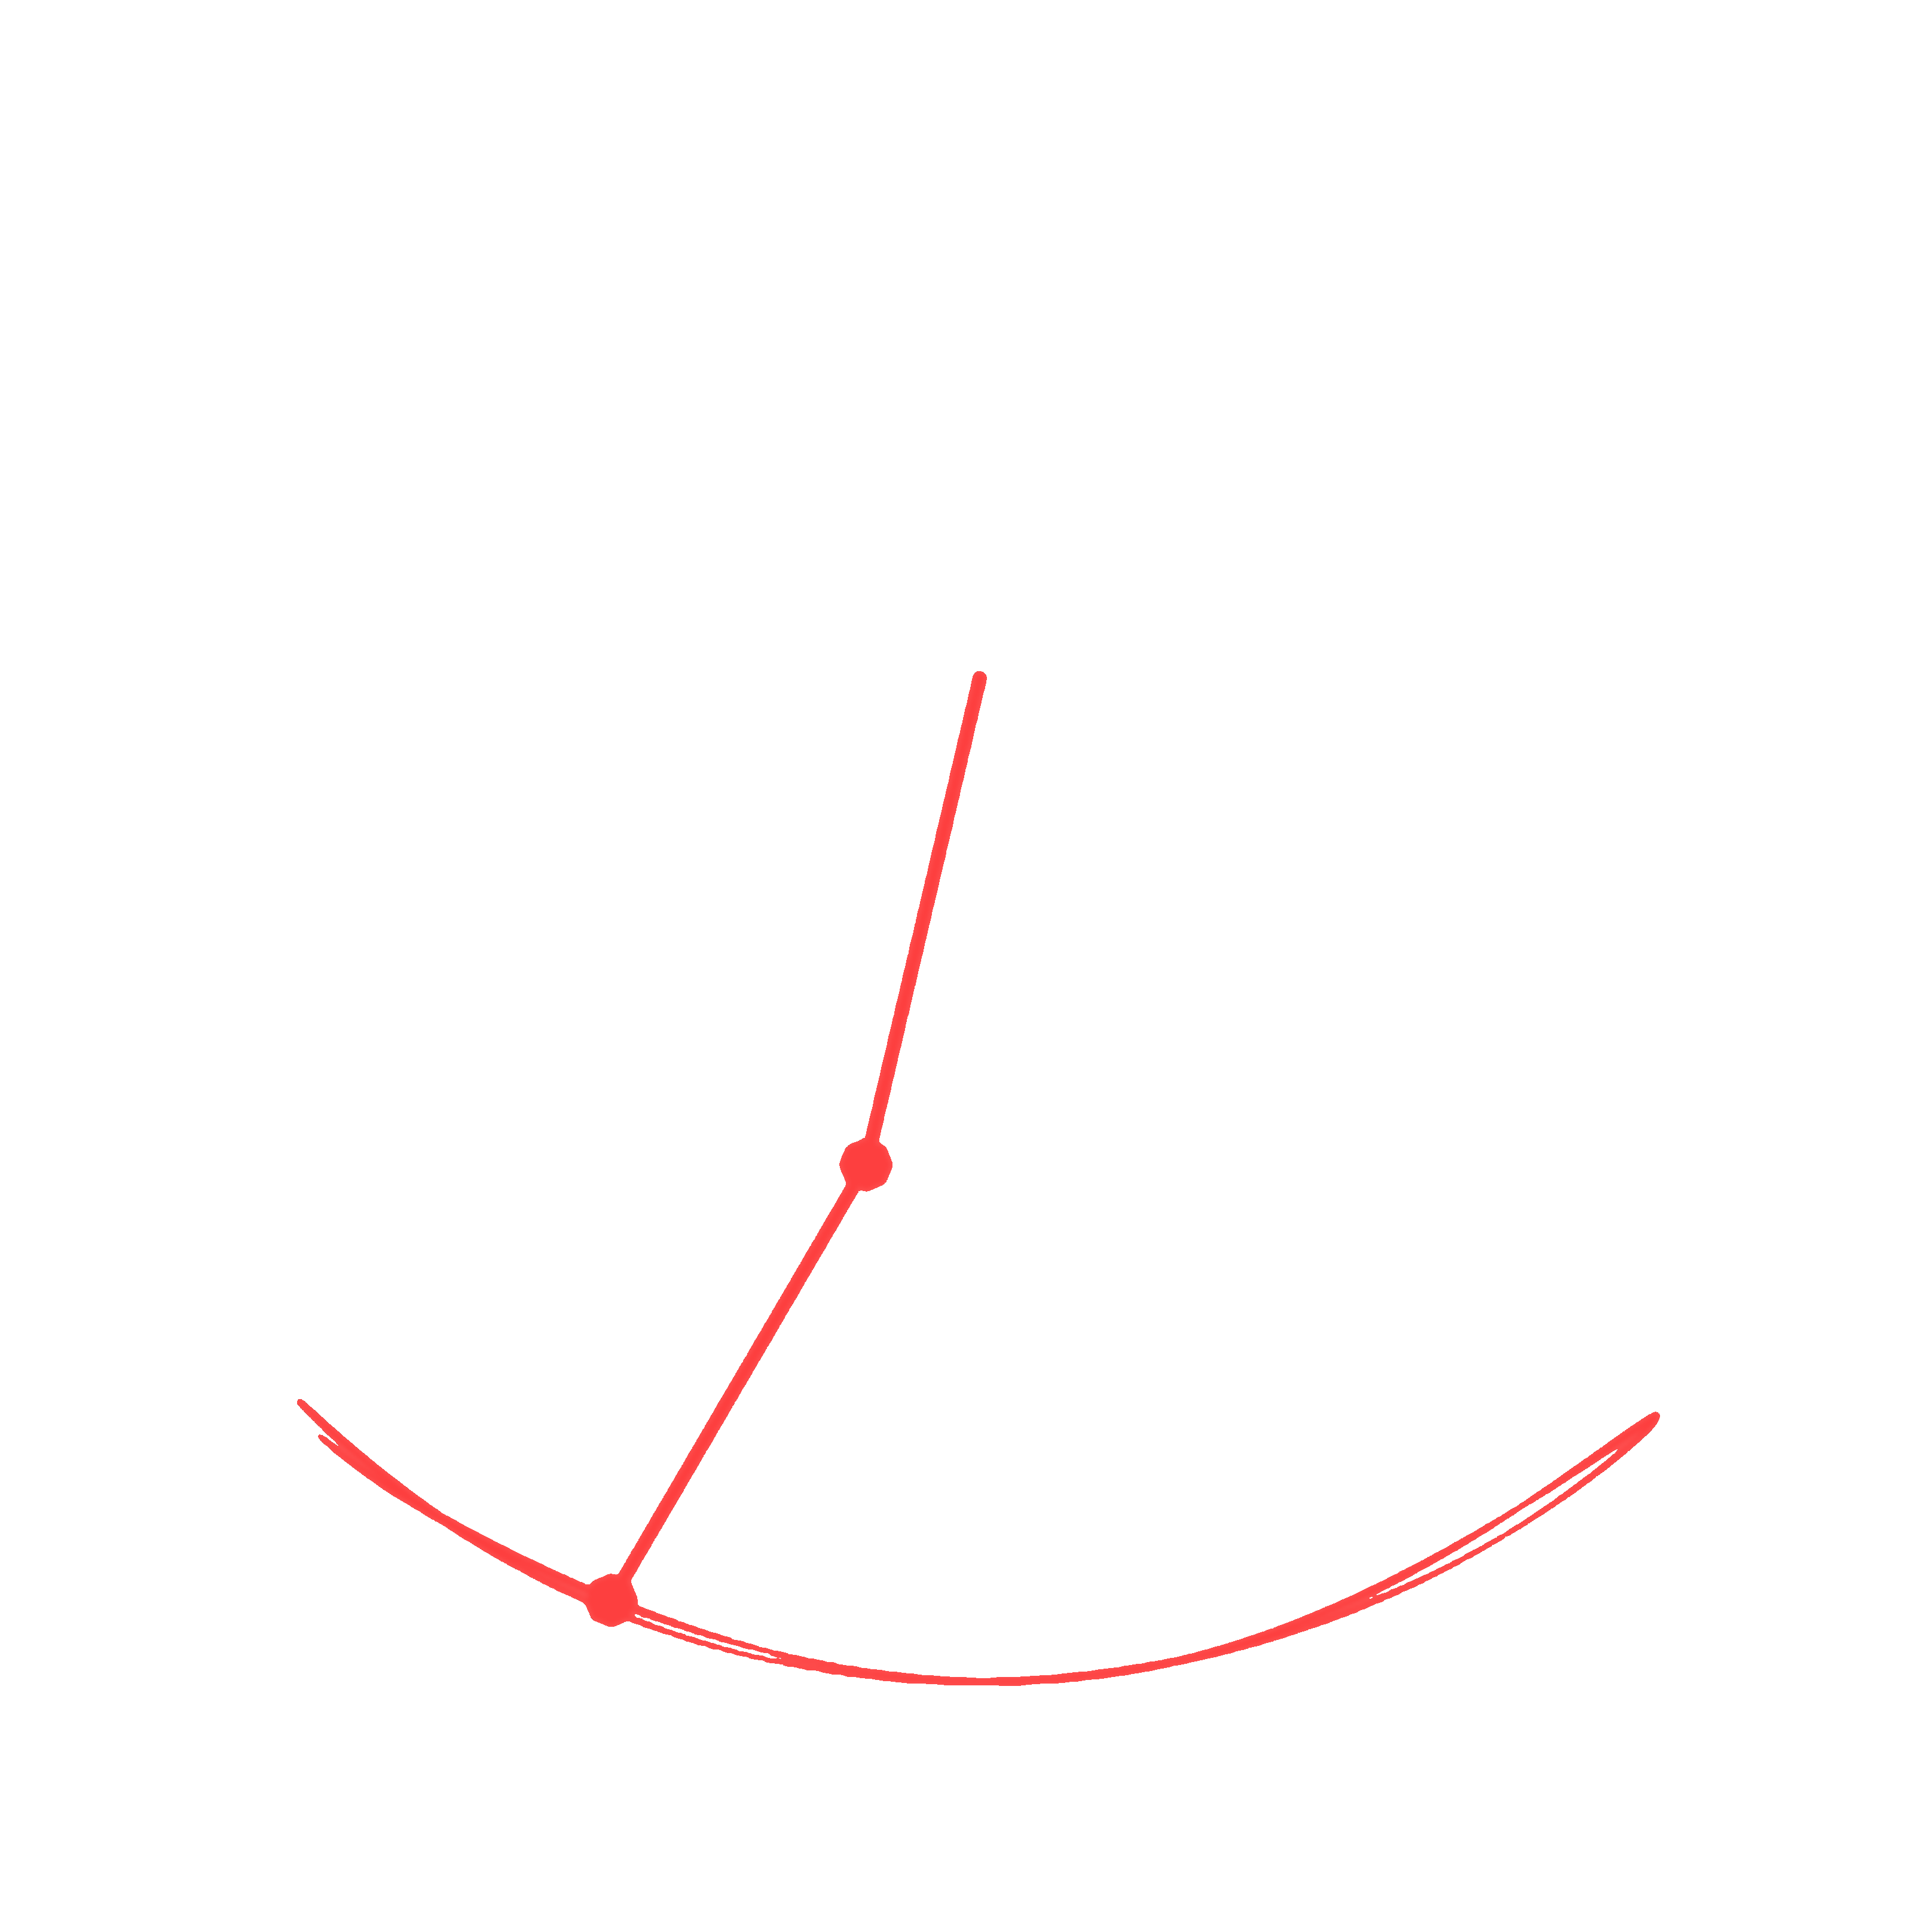
\includegraphics[width=\textwidth]{papers/doppelpendel/images/pendel_spur_nichtchaotisch.png}
    \end{minipage}
    \caption{Pendel wird nicht chaotisch, aufgrund kleiner Winkel.}
    \label{fig:pendel_nichtchaotisch}
\end{figure}
